%Preámbulo
\documentclass[11pt,titlepage]{report}
\usepackage[spanish]{babel}
\usepackage[utf8]{inputenc} 
\usepackage[T1]{fontenc}
\usepackage{lmodern}
\usepackage[tmargin =1.25in, lmargin=1.25in, rmargin=1.25in, bmargin=1.25in]{geometry}
\usepackage{placeins}
\usepackage{graphicx}
\usepackage{titlesec}
\usepackage[table,xcdraw]{xcolor}
\usepackage{rotating}
\usepackage{float}
\usepackage{subfig} %dos figuras juntas
\usepackage{lscape}
\usepackage{wrapfig} %se escribe a la par de la figura
\usepackage{fancyhdr}
\pagestyle{fancy}
\usepackage{cite}
\usepackage{amsmath}
\usepackage{caption}
\usepackage{chronosys}

% encabezados
\lhead[\thepage]{\rightmark}
\chead[]{}
\rhead[CAPÍTULO \thechapter. \leftmark]{\thepage}
\renewcommand{\headrulewidth}{0.5pt}

% pie de pagina
\lfoot[]{REDES NEURONALES}
\cfoot[]{}
\rfoot[Lester Vallecillo]{UNAH}
\renewcommand{\footrulewidth}{0pt}

\title{UN BREVE ESTUDIO DE REDES NEURONALES}
\author{Lester Armando Vallecillo M.}
\date{12 de Diciembre del 2019}
\renewcommand{\headrulewidth}{0.4pt} % grosor de la cabecera
\usepackage{chngcntr}
\counterwithout{footnote}{chapter}
%cuenta todos los indices sin empezar un nuevo conteo en el siguinete capitulo

% ****************************************************

%definir condiciones de estilo del documento
\renewcommand{\baselinestretch}{1.5} %Interlineado 1.5
\rm %definir el tipo de letra en Roman

\titleformat{\chapter}{\normalfont\huge}{\thechapter.}{14pt}{\huge\it}
  
%\renewcommand*\thesection{\arabic{section}}
%\renewcommand*\thesubsection{\arabic{subsection}}
\begin{document}
	


%%%%%%%%%%%%%%%%%%%%% portada %%%%%%%%%%%%%%%%%%%%%%%%%%%%%%%%%%%%%%%%%%
\begin{titlepage}
  \vspace*{1cm}
\begin{center}
  		\Huge{\textbf{UN BREVE ESTUDIO DE REDES NEURONALES}}
\end{center}
\vspace*{1cm}
    
    % Línea gris
\hrule
  
 \begin{center}
	{\LARGE{UNIVERSIDAD NACIONAL AUTÓNOMA DE HONDURAS}}\\
	{\LARGE \textbf{Carrera de Matemáticas}}\\[0.4cm] 
 	
\includegraphics[height=6cm]{Pic/UNAH}\\[0.3cm]
 	{\LARGE\underline{ Seminario de Investigación}}\\ 
 \end{center}
\begin{center}
	\begin{list}{}{}
	\item \begin{center}
		\textbf{Autor:}
	\end{center}
	\item \begin{center}
		Lester Armando Vallecillo
	\end{center}
	\item \begin{center}
		\textbf{Supervisor:}
	\end{center}
	\item \begin{center}
		Dr. Jorge Arturo Destephen\\[1.5cm]
	\end{center}
\end{list}
\end{center}
   {\large Tegucigalpa, Honduras, C.A. \hfill 11 de Diciembre del 2019}
\end{titlepage}


%%%%%%%%%%%%%%%%%%%%%%% ABSTRACT %%%%%%%%%%%%%%%%%%%%%%%%%%%%%%%%%%%%%%%
\begin{abstract}
La aplicación de la inteligencia artificial permite abrir paso a una de las herramientas mas importantes para el análisis de datos, denominado Red Neuronal Artificial(ANS\footnote{Por sus siglas en ingles, Artificial Neural Systems.}), este modelo fue inspirado por el sistema neuronal biologico(BNS\footnote{Por sus siglas en ingles, Biological Neural Systems.}). Surge con la necesidad de modelar problemas lineales y no lineales de diferentes áreas de estudio para obtener resultados mas precisos y automatizar los cálculos de la solución. Dicha herramienta es una familia de algoritmos de aprendizaje automatizado\footnote{Conocido como Machine Learning, por sus siglas en ingles. Es una rama de la inteligencia artificial.} mas populares que se utiliza con frecuencia en problemas de predicción y clasificación obteniendo un alto grado de precisión.\\  

El propósito de estudio es comprender los aspectos teóricos y prácticos relacionados con ANS, para modelar problemas lineales y no lineales, particularmente en una aplicación del campo de las finanzas, denominada aprobación de crédito. De la misma manera, se pretende evaluar la capacidad de la red en la predicción de problemas de clasificación, comparando la medida del error obtenido en el entrenamiento de las redes neuronales mas utilizadas.\\

En la comparación de resultados de la aplicación de las redes Perceptrón Multicapa(MLFN) de 2 a 6 nodos y una red neuronal probabilística(PNN) a el problema de aprobación de crédito, se selecciona PNN como el tipo de red para modelar este problema porque tiene el mínimo error global, dando un aporte a la solución, ya que no solo clasifica, ademas determina la probabilidad del error en la predicción. Por su parte, se espera que el 9.2\% de las predicciones serán incorrectas para los nuevos solicitantes de crédito.\\
              
\paragraph{Palabras Clave:}	
Inteligencia artificial, aprendizaje automático, Modelo, Predicción, Problemas de clasificación, Técnicas de aprendizaje, propagación.

	
\end{abstract}
\pagenumbering{roman}

\tableofcontents

\chapter*{Introducción}
Con el avance de la tecnología, las redes neuronales se vuelven cada día mas importantes por su aprendizaje profundo\footnote{Conocido como deep learning, por sus siglas en ingles. Es un conjunto de algoritmos de aprendizaje automático que intenta modelar abstracciones de alto nivel en datos.\cite{Int08}}, es una herramienta para el análisis de datos que pertenece a un nuevo campo de estudio conocido como ciencia de datos\footnote{Conocido como data science. Es un campo de métodos científicos.} con la finalidad de extraer conocimiento de los datos. Sin embargo, esta herramientas surge de forma paralela con la aparición de los primeros computadores, desde ese entonces, son utilizados para modelar neuronas individuales \cite{Lib03}.\\

 En fin, hay muchas tareas que resultan especialmente adecuadas para ser resueltas mediante computadores, y así, obtener la resolución de problemas reales simulando procesos ó eventos que se pueden modelar matemáticamente. Ciertamente, hay muchas aplicaciones que desearíamos automatizar, pero esta necesidad requiere en algunos casos de generar inteligencia artificial, en cuyo problema aparece como propuesta el modelo ANS, que básicamente emula la inteligencia de sistema biológico(BNS) implícito en el cerebro humano. En consecuencia de esté modelo, surgen algunos estudios, que fundamentan los aspectos teóricos relacionados a el aprendizaje automatizado, se describen en una linea de tiempo, a continuación:  

\begin{figure}[h]
	\caption{Línea de tiempo}
	\centering
	\resizebox{\linewidth}{!}{% Resize table to fit within
		
		\begin{tikzpicture}[]
		%draw horizontal line
		\draw (0,0) -- (41/1.7,0);
		%draw vertical lines
		\foreach \x in {0, 6, 13, 20, 27, 35}{
			\draw (\x/1.7,3pt) -- (\x/1.7,-3pt);
		}
		%draw nodes
		\draw (0,0) node[below=3pt]{\textbf{ARN}} node[above=3pt]{1943(McCulloch-Pot)};
		\draw (8/1.7,0) node[below=3pt] {\textbf{Computador}} node[above=3pt]{1950(Turing)};
		\draw (15/1.7,0) node[below=3pt] {\textbf{Análisis exploratorio}} node[above=3pt] {1977(Tukey)};
		\draw (22/1.7,0) node[below=3pt] {\textbf{Minería de datos}} node[above=3pt] {1996(Fayyad-Piatetsky)};
		\draw (29/1.7,0) node[below=3pt] {\textbf{Ciencia de datos}} node[above=3pt] {2001(Cleveland)};
		\draw (36/1.7,0) node[below=3pt] {\textbf{Deep learning}} node[above=3pt] {2013(Bengio, A. Courville)};
		
		\end{tikzpicture}
	}
	\label{fig:time_line}
\end{figure}

En 1981, el Dr. White realizó un trabajo que ilustraba el uso de ANS en la predicción de variables financieras. Desde entonces, se ha incrementado el estudio de las aplicaciones de ANS en el campo de las finanzas \cite{Rev19}. Entre las cuales se destacan la Predicción de índices, detección de fraudes, riesgo crediticio, clasificación y predicción de la rentabilidad de acciones. Mientras tanto, en el área de negocios: Marketing, venta cruzada y campañas de venta. En tratamientos de texto: Reconocimiento de caracteres, gráficos y escritura. En el área de Alimentación: Análisis de olor y aroma, perfilamiento de clientes, desarrollo de productos y Control de calidad. En el área de Energía: Predicción del consumo eléctrico y Distribución recursos hidráulicos para la producción. En el área Eléctrica: Predicción consumo de gas ciudad, industria manufacturera, control de procesos, control de calidad y control de robots. En medicina y salud: Ayuda al diagnóstico, análisis de imágenes, desarrollo de medicamentos y distribución de recursos. En ciencias e ingeniería: Análisis de datos, clasificación, ingeniería química, ingeniería eléctrica y climatología. En transportes y comunicaciones: Optimización de rutas y optimización en la distribución de recursos \cite{Art13}.\\

Algunos estudios afirman que las ANS son eficientes a la hora de esperar buenos resultados en muchos tipos de problemas de clasificación, porque son capaces de predecir variables dependientes categóricas de manera precisa, mejorando la solución de métodos tradicionales de predicción como los modelos ARIMA y la regresión lineal entre otros, agregando las variantes de aprendizaje automático, solución de problemas no lineales con un alto grado de precisión y captura de correlación entre las variables de algún conjunto de datos.\\

El Capitulo 1, se centra en describir los fundamentos teóricos de la estructura y funcionalidad de ANS. De la misma manera, en el Capitulo 2, se pretende evaluar la capacidad de solución para un problema de clasificación, estudiando una aplicación particular del campo de las finanzas. En el capitulo 3, se analizan el resultado final de la aplicación de ANS para validar la red neuronal, determinando el mejor tipo de red con la medida del mínimo error absoluto en la predicción del entrenamiento de la red. De esta manera, se selecciona la red neuronal mas adecuada utilizando un software, para modelar el problema de clasificación que se presenta, denominado Análisis de crédito.
%%%%%%%%%%%%%%%%%%%%%%%%%%%%%%%%%%%%%%%%%%%%%%%%%%%%



%%%%%%%%%%%%%%%%%%%%%%%%%% FUNDAMENTOS TEORICOS  $$$$$$$$$$$$$$$$$$$$$$$$$$$$$$$$
\chapter{Fundamentos Teóricos} 
\pagenumbering{arabic}
El cerebro humano consiste en billones de neuronas biológicas interceptadas. Su estructura esta definida de tal manera que, el axón(salida) de la neurona se ramifica y está conectada a las dendritas(entradas) de otras neuronas a través de uniones llamadas sinapsis\footnote{Es una aproximación funcional intercelular.}. La teoría de las ANS esta basada en este modelo básico del cerebro humano, denominado BNS \cite{Art01}. Para mostrar la relación existente entre ambos modelos primero definimos los conceptos del modelo BNS, el cual sera el prototipo\footnote{Se refiere a un objeto que sirve como modelo para la construcción de un nuevo objeto.} para fundamentar la teoría del modelo ANS, su metodología se describe en el diagrama siguiente:

\begin{figure}[h] 
\centering	
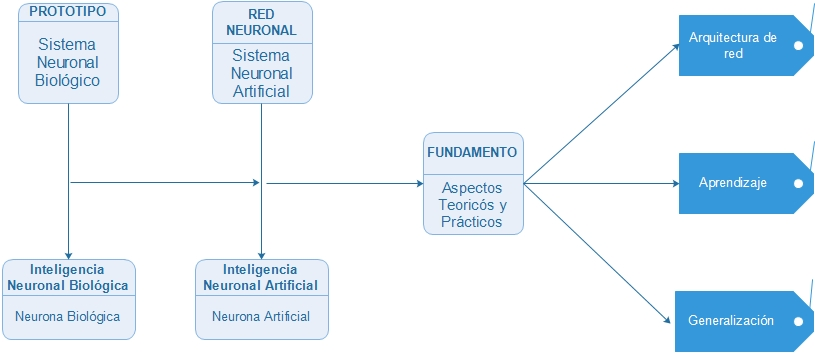
\includegraphics[scale=0.7]{Pic/Diagrama01} 
\label{Diagrama01}.
\caption{Metodología de Definicion de Red Neuronal Artificial. [Fuente: propia]}
\hrule
\end{figure}

\section{Neurona biológica}
Son células nerviosas que constituyen los elementos primordiales del sistema nervioso central. Una neurona es capaz de recibir información de miles de otras neuronas, procesarla y luego generar una nueva información que enviará a otras neuronas con las que está conectada. Se estima que el cerebro está compuesto por más de 10 billones de neuronas y que cada una está conectada a más de 10 mil neuronas. Una neurona biológica está compuesta por: cuerpo celular o soma, axón y dendritas.\\  

\begin{figure}[h] 
	\centering	
	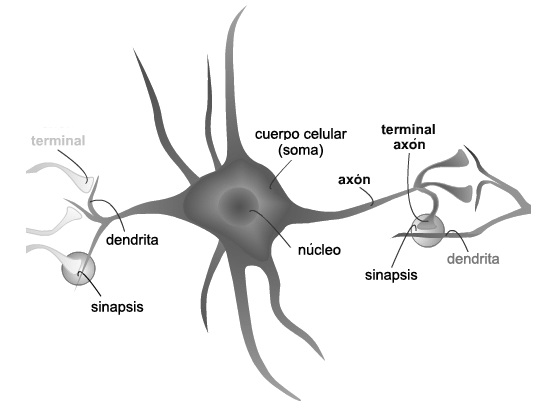
\includegraphics[scale=0.8]{Pic/neuronabiologica03}
	\caption{Esquema de una neurona biológica. \cite{Int10} }
	\hrule
\end{figure} 
%%%%%%%%%%%%%%%%%%%%%%%%%%%%%%%%%%%%%%%%%%%%%%%%%%%%%%%%%%%%%%%

\section{La unión sináptica}
Desde el cuerpo de una neurona se extienden las dendritas hacia otras neuronas donde reciben las señales transmitidas por otras neuronas. El punto de contacto o de conexión se denomina unión sináptica o sinapsis. La comunicación entre ellos da como resultado la liberación de unas sustancias llamadas neurotransmisores por parte de las células \cite{Lib06}.
%%%%%%%%%%%%%%%%%%%%%%%%%%%%%%%%%%%%%%%%%%%%%%%%%%%%%%%%%%%%%%%%%555

\section{Sistema Neuronal Biológico(Prototipo)}
El sistema neuronal biológico(BNS) se utiliza como prototipo para construir los fundamentos del sistema neuronal artificial(ANS), inspirado en la estructuración del cerebro humano. El sistema nervioso esta constituido por neuronas interceptadas entre si, presenta una estructura compleja compuesta por neuronas biológicas. El promedio de neuronas es de $10^{11}$ y las conexiones promedio entre ellas son de orden maximo de $10^{15}$ \cite{Art14}. La analogía del comparativo entre ambos sistemas, se resume en la tabla siguiente: 

\begin{figure}[h]
	\centering
	\subfloat{
		\begin{tabular}{| l | r |} \hline
			\textbf{Ordenador} & \textbf{Cerebro humano}\\ \hline
			Computación en serie & Computación en paralelo\\ \hline
			Poco robusto & Tolerancia a fallos\\ \hline
			Programable & Aprendizaje autónomo\\ \hline
			Digital & Analógico\\ \hline
			$10^{9}$ transistores &  $10^{15}$ sinapsis\\ \hline
			$3.6GHz$ Nanosegundos & $4\sim90Hz$ Milisegundos\\ \hline
			51.2 GB/s & 10 spikes/s\\ \hline
			210,000,000 m/s & $1 \sim100 m/s$\\ \hline
			$2.3x10^{13}$ TEPS & $6.4x10^{14}$ TEPS\\ \hline
	\end{tabular}} \caption{Analogía entre ambos sistemas.\cite{Art14}}
	\subfloat{
		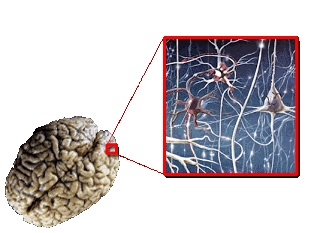
\includegraphics[width=0.45\textwidth]{Pic/Cerebroneurona02}}
	\caption{Fabian N.(2010). Estructura del sistema neuronal biológico. \cite{Int09}}
	\hrule
\end{figure}

Las neurona tienen propiedades particulares diferentes como recibir, procesar y transmitir señales electroquímicas a través de todas las conexiones del sistema de comunicación del cerebro. Basado en este prototipo, se define la neurona artificial como el componente principal de ANS.
%%%%%%%%%%%%%%%%%%%%%%%%%%%%%%%%%%%%%%%%%%%%%%%%%%%%%%%%%%%%%%%%%%%%%

\section{Neurona Artificial}
Una neurona artificial es una abstracción de una neurona biológica y su función principal es el procesamiento de información, el cual es la componente fundamental para la estructura y funcionalidad de una ANS. Una neurona artificial está compuesta por: un conjunto de entradas, un conjunto de pesos sinápticos, un cuerpo celular y una salida, como se muestra en la figura siguiente: 

\begin{figure}[h]
	\centering
	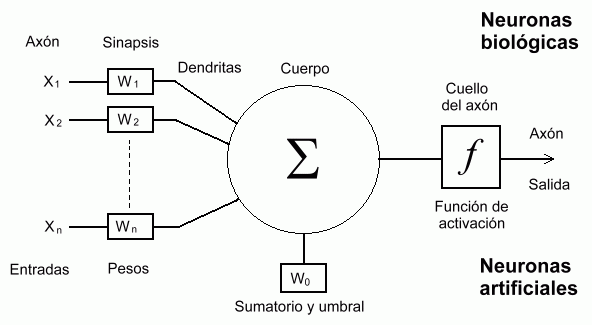
\includegraphics[scale=0.7]{Pic/03-SA} 
	\caption{Modelo neuronal de McCulloch-Pitts.\cite{Int11}}
	\hrule
\end{figure}
Una representación del funcionamiento básico de una neurona artificial, es semejante a la regresión lineal, que aproxima la relación de dependencia entre las variables independientes, los elementos principales son:
\subsection{Entradas(Axón)}
Son los valores $X_i$ para $i=1,2,3, .., n$, que representan las variables de entrada en los datos.

\subsection{Pesos(Sinapsís)}
Son los valores $W_i$ que representan las pesos sinápticos de las variables en una neurona.


\subsection{Función Suma(Cuerpo)}
Es la sumatoria de los valores de entradas multiplicados por su peso sinápticos. Se describe en la ecuación siguiente:
\[ S(U, W_1, W_2, .., W_n) = \sum^{n} X_i W_i + U\]
Donde $X_i$ son las entradas, $U$ el umbral y $W_i$ los pesos sinápticos.

Este funcionamiento es limitado a problemas lineales, por lo tanto, para aproximar la relación de dependencia entre variables de problemas no lineales, es necesario, la composición de neuronas y de esta manera, romper el esquema de linealidad. En consecuencia, la composición de neuronas o red neuronal, puede arrastrar el mismo problema de la linealidad, a esto se le llama colapso de la red, porque el resultado es similar a aproximar una función con la regresión lineal. Como solución al problema, se propone evaluar la variables de entrada de las neuronas y su umbral en la función de activación.      

\subsection{Función de activación(Cuello de axón)}
Es la función $f(S)$ que evalúa la función suma, para determinar el potencial de activación de la neurona. Se buscan funciones que las derivadas sean simples, para minimizar con ello el coste computacional. Por ejemplo:
\subsubsection{Función Sigmoide}
En general, una función sigmoide es un función real de variable diferenciable, de la forma: \hspace{1cm} $f(x)= y = \frac{1}{1+e^{-x}} $\\
La primera derivada es: $y' = \frac{e^{-x}}{(1+e^{-x})^{2}}$, de donde, $y' = y(1-y)$.

\subsection{Salida}
Son los valores de salida $y_i$ de la neurona, que devuelve la función de activación y evalua el error con respecto del valor esperado por medio de una función de red.

%%%%%%%%%%%%%%%%%%%%%%%%%%%%%%%%%%%%%%%%%%%%%%%%%%%%%%%%%%%%%%%%%%
\subsection{Interconexiones(Dentritas)}
Con el objetivo de construir el modelo ANS, se define una red compuesta por neuronas artificiales mediante múltiples interconexiones, de manera similar a cerebro humano(BNS).
%%%%%%%%%%%%%%%%%%%%%%%%%%%%%%%%%%%%%%%%%%%%%%%%%%%%%%%%%%%%%%%%
\section{Redes Neuronales Artificiales(ANS)} 
Una ANS es una red compuesta por neuronas artificiales que están interceptadas de alguna manera y trabajan para poder simular un problema específico. Generalmente, están estructuradas por capas de nodos que envían y reciben respuestas entre si, similar a la manera en que el cerebro procesa la información. El resultado de la respuesta de salida es comparada con la esperada para calcular el error hasta ser minimo. Ver en la siguiente figura \ref{01}, su esquema de funcionalidad. 
%%%%%%%%%%%%%%%%%%%%%%%%%%%%%5
\subsection{Definición}
\textit{Una Red Neuronal es un conjunto de nodos interconectados, que realizan al menos una de las siguientes funciones: Aprendizaje, Memorización, Generalización o Abstracción de características a partir de un conjunto de datos \cite{Lib03}.} 
\begin{figure}[h]
	\centering
	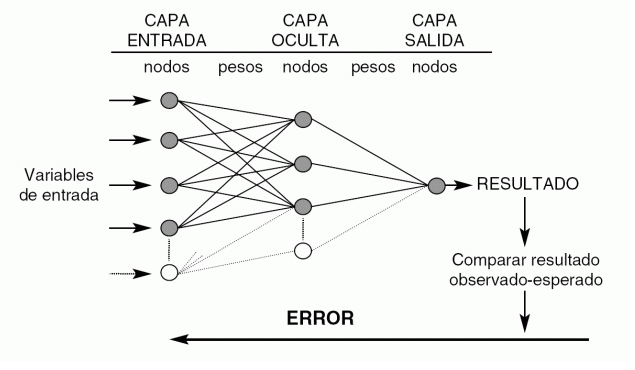
\includegraphics[scale=0.8]{Pic/04-RA}
	\caption{Esquema de una Red Neurona Artificial.\cite{Lib12}}
	\label{01}
	\hrule
\end{figure}

\subsection{Función de error} 
Es una función $E(y))$ que evalúa el error entre el valor estimado y el valor real de salida. Por ejemplo: La función Error cuadrático medio.

\subsection{Función de red}
También conocida como función de coste. Modifica los pesos sinápticos de la red mediante la derivada parcial de una composición de funciones $E(f(S(U, W_1, W_2, .., W_n)))$, con el propósito de minimizar el error en los valores de las salidas. Es decir, se puede modificar el peso sináptico de cada variable en función del error de salida, de la forma siguiente:

\[\dfrac{ \partial E}{\partial W_i} = \dfrac{ \partial E}{\partial f}\dfrac{ \partial f}{\partial S}\dfrac{ \partial S}{\partial W_i} \]

Si $f(W_i)$ es un vector de n predicciones y $Y$ es el vector de los valores esperados, entonces el estimado $E_2$ del predictor es: \cite{Int08}

\[E_2 =\frac{1}{n}\sum_{i=1}^{n}(f(W_i)-Y_{i})^{2}\]

Su derivada minimiza el coste computacional, $ \dfrac{\partial E_2}{\partial f(W_i)} = f(W_i) - Y_i $\\
 
%%%%%%%%%%%%%%%%%%%%%%%%%%%%%%%%%%%%%%%%%%%%%%%%%%%%%%%%%%%%5

En el estudio de las ANS se consideran tres aspectos fundamentales: La arquitectura, el aprendizaje y la capacidad de generalización de la red \cite{Lib04}.


\section{Arquitectura de red}
Es el diseño estructural de la red, relacionado al problema que se pretende modelar y busca determinar los siguientes elementos: \label{08}
\begin{description}
	\item[1. Entradas y salidas:] Se determina la cantidad de entradas y salidas.
	 
	\item[2. Nodos ocultos:] Se refiere al numero de capas ocultas formadas por las neuronas que se encuentran entre los nodos de entrada y de salida.  
	\item[3. Función de red:]  Esta función penaliza la red para modificar los pesos sinápticos mediante un proceso de aprendizaje. 
	 
	\item[4. Función de activación:] devuelve una salida a partir de un valor de entrada, normalmente la salida tiene un valor en un rango determinado como $(0,1)$ ó $(-1,1)$.
	
	\item[5. Interconexión entre nodos:] La forma en que los nodos están interconectados.
	\item[6. Propagación de red:] La dirección que sigue la información 
	\item[7. Selección de datos:] Con la selección de un conjunto de datos adecuado se realizar el entrenamiento\footnote{Significa seleccionar un modelo de la serie de modelos permitidos}  y de esta manera se valida el modelo del problema.
\end{description}

\section{Aprendizaje}
Es el proceso\footnote{Consiste en representar un conjunto de datos como conjunto de patrones de entrenamiento.} en el cual los pesos sinápticos son modificados con el objetivo de capturar la información que se presenta, y así obtener respuestas mas precisas. Normalmente el proceso se realiza hasta que se produce un evento de los siguientes:

\begin{itemize}
	\item El error entre la salida de la red y la deseada alcance un valor aceptable.
	\item  Se alcance el número máximo de ciclos.
\end{itemize}
	
El aprendizaje se lleva a cabo mediante el uso de algoritmos de entrenamiento. Por ejemplo, en Anexo \ref{09}, se presenta un esquema del algoritmo backpropagatión.


%%%%%%%%%%%%%%%%%%%%%%%%%%%%%%%%%%%%%%%%%%%%%%%%%%%%%%%%%%%%%%%%%%%%%%
\section{Generalización}
La capacidad de generalización de una red esta asociada a la recuperación de información que es almacenada en los pesos sinápticos de las conexiones durante el entrenamiento, evaluando así, los resultados de un conjunto de datos utilizados en el proceso de aprendizaje. Se espera que cuando se presenten patrones que no han sido enseñados a la red, ésta sea capaz de entregar una respuesta cercana a la deseada. 

%%%%%%%%%%%%%%%%5 CLASSIFICACION DE REDES NEURONALES %%%%%%%%%%%%%%%%%%%%%%%%%%%%%%%%%%%%%%
\section{Clasificación de redes neuronales}
La mayoría de las aplicaciones de redes neuronales se pueden clasificar en aplicaciones de Predicción, Clasificación, Asociación, Conceptualización, Filtrado y Optimización \cite{Art02}. Por su funcionalidad se pueden clasificar de la forma siguiente:

\subsection{Según su arquitectura}
Consiste en la organización de las neuronas. Las neuronas se agrupan formando capas de diferentes características. Algunos ejemplos comunes son:
\begin{center}
	\begin{description}
		\item[a. Perceptrón simple]  Esta compuesta por una capa.
		\item[b. Perc. Multicapa] Dispone de un conjunto de capas.
		\item[c. Convolucional] Se une con un subconjunto de capaz.
		\item[d. Recurrente] Permite conexiones arbitrarias.
		\item[e. Base radial] Calculan la salida de la función.\\[1cm]
\end{description}
\end{center}

\subsection{Según su aprendizaje}
 Consiste en algoritmos basados en formulas matemáticas que usando técnicas modifican el valor de los pesos sinápticos y con ello optimizan la respuesta de salida de la red. Se subdivide en:
	
\subsubsection{Aprendizaje Supervisado}
Es el proceso en el cual se realiza un aprendizaje con un entrenamiento controlado. Algunos ejemplos destacados, son los siguientes:
	\begin{description}
		\item[1. Corrección del error] Ajusta los pesos de las conexiones en función del error. Entre los mas utilizados, tenemos los siguientes ejemplos:
		\begin{itemize}
			\item Perceptrón
			\item Mínimo error cuadrado
			\item Propagación hacia atrás
		\end{itemize}
		\item[2. Estocástico] Realiza cambios aleatorios, tomando los mejores resultados.  
		
	\end{description}
\subsubsection{Aprendizaje No Supervisado}
	No requiere influencia externa para ajustar los pesos.  Algunos ejemplos destacados, son los siguientes:
	\begin{description}
		\item[1. Hebbiano]	 Extrae características de las entradas.
		\item[2. Comparativo] Clasifica las entradas de la red.	          
	\end{description}
\subsubsection{Aprendizaje Por refuerzo} El usuario indica cuando los datos son aceptables o no, según sus propios criterios al hacer observaciones. El proceso del aprendizaje por refuerzo consiste en determinar las siguientes componentes:
\begin{itemize}
\item Un conjunto de estados
\item Un conjunto de acciones
\item Reglas de la transición entre los estados
\item Reglas de recompensa escalar de una transición
\item Reglas que describen lo que observa el agente
\end{itemize}

La observación implica típicamente la recompensa inmediata al escalar asociado con la última transición \cite{Int08}.

%%%%%%%%%%%%%%%%%%%%%%%%% ESTRUCTURA DE ALGUNAS REDES  %%%%%%%%%%%%%%%%%%%%%%%%%%%%%%%%%%
\section{Ejemplos de arquitectura de ANS}
\subsection{Perceptrón y Adaline}
El adaline \footnote{Por sus siglas en ingles, Adaptative Linear Element} está basado en la Neurona de McCulloch-Pitts(Perceptrón). 
La diferencia entre Perceptrón y Adaline, que para modificar los pesos sinápticos, Adaline toma en cuenta la corrección de la salida estimada respecto al valor deseado. En la Figura \ref{03}, se muestra una comparación entre ambas arquitecturas de red \cite{Int08}.
\begin{figure}[h]
	\centering
	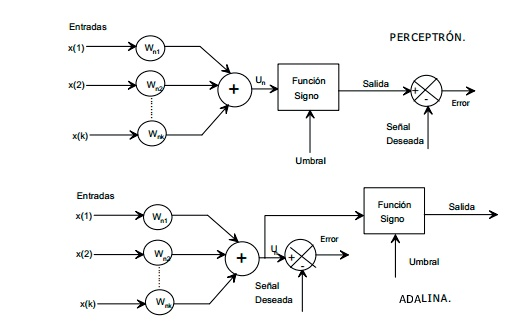
\includegraphics[scale=1]{Pic/red02}
\caption{Comparación de la estructura de la red Perceptrón y Adaline.\cite{Lib04}}
\label{03}
\hrule
\end{figure}

\subsection{Perceptrón multicapa(MLFN)}
El perceptrón multicapa(MLFN\footnote{Por sus siglas en ingles, multilevel forward networks}) es una red formada por múltiples capas interconectadas hacia adelante y tiene como función de red el algoritmo backpropagatión. En la figura \ref{04}, se muestra su arquitectura de red.
\begin{figure}[h]
	\centering
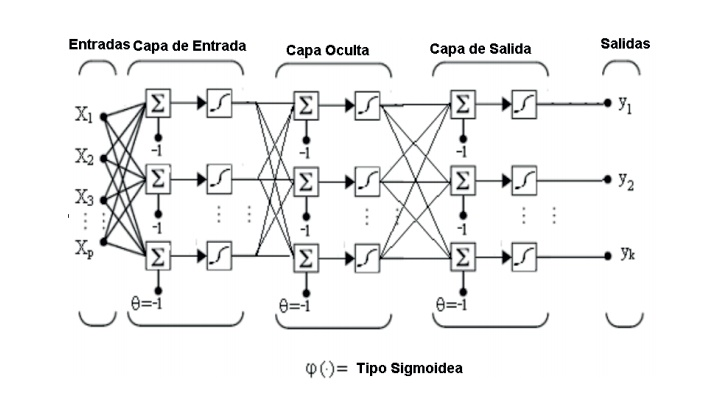
\includegraphics[scale=0.78]{Pic/red03}
\caption{Perceptrón multicapa, utilizando una funciones de salida Sigmoide. \cite{Lib04}\\}
\label{04}
\hrule
\end{figure}
\newpage
\subsubsection{Backpropagatión(regla delta)}
Es el algoritmo mediante el cual la función de coste modifica el valor de los pesos entre las conexiones de las neuronas mediante la propagación hacia atrás, desde la capa de salida hacia la capa de entrada, a través de las capas ocultas. En la Figura \ref{02}, se puede ilustrar como se propaga dicha función.\\
\begin{figure}[h]
\centering
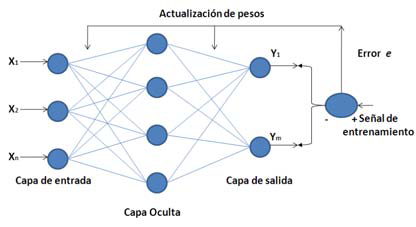
\includegraphics[scale=0.7]{Pic/Backpropagation}
\caption{Esquema de propagación hacia atrás.\cite{Int10}}
\label{02}
\hrule
\end{figure}

\subsubsection{Proceso de entrenamiento: Backpropagatión} 
El proceso de aprendizaje se describe en los pasos siguientes:

\begin{enumerate}
\item Se inician los pesos con valores aleatorios.
\item Se presenta un patrón n de entrenamiento $\{X(n), S(n)\}$, se evalúa en propagación hacia adelante y se obtiene respuesta de la red $Y(n)$.
\item  Se evalúa el error que comete la red para cada neurona.
\item Se modifican los pesos de la red con la propagación hacia atrás.
\item Se repite el proceso hasta alcanzar un mínimo de error.
\end{enumerate}

Este proceso es un aprendizaje supervisado por corrección del error mediante una función de coste que penaliza la red, su algoritmo se ilustra de una forma mas clara en Anexo 1, Figura \ref{09}. 

\subsection{Comparación de redes MLFN y PNN}
Cada uno de los tipos de ANS tiene ventajas, las cuales se describen, a continuación:
\subsubsection{Ventajas de MLFN}
\begin{itemize}
	\item Más rápidas para hacer predicciones.
	\item Son más fiables fuera del rango de los datos de entrenamiento.
	\item Son capaces de generalizar a partir de conjuntos de entrenamiento
	pequeños.
\end{itemize}

\subsubsection{Ventajas de PNN}  
\begin{itemize} 
	\item Se entrenan rápido.
	\item No requieren una especificación de arquitectura.
	\item Las redes PN no sólo clasifican, sino que también generan
	probabilidades de que el caso se encuentre en diferentes categorías dependientes posibles. \cite{Guia17}
\end{itemize}
%%%%%%%%%%%%%%%%%%%%%%%%%%%%%%%%%%%%%%%%%%%%%%%%%%%%%%%%%%%%%%%%%%%%%%%

\subsection{Redes neuronales probabilísticas(PNN)}

Una red neuronal probabilística(PNN\footnote{Por sus siglas en ingles, probabilistic neural network}) es una red unidireccional y semisupervisada que pertenece a la familia de redes neuronales con función de base radial y es a menudo utilizadas en problemas de clasificación. Una red PNN es capaz de estimar límites o superficies de decisión no lineales mediante un enfoque óptimo Bayesiano.\\

A diferencia del proceso de aprendizaje que se lleva a cabo en la mayoría de las ANS, en el cual se realiza un ajuste a los valores de los pesos sinápticos $W_i$, para hacer uso de una PNN no es necesario realizar ningún ajuste de pesos y sólo se determina a los patrones de salida mediante la comparación y el cálculo de las distancias de cada uno de los patrones ejemplo o vectores de datos de entrada, a través de la función $\varphi_{ij}$, utilizado como la función de activación \cite{Art15}. Como se muestra en la ecuación siguiente \cite{Art16}:

\[ \varphi_{jk} = \dfrac{1}{(\sqrt{2\pi}\sigma)^d} \exp{(-\dfrac{1}{2\sigma^2})(x-{m_{jk}}^x)^2} \]
\label{10}
Donde $x$ el vector de entradas, $d$ es el tamaño del vector, ${m_{jk}}^x$ es el j-enésimo vector de referencia, $k$ es la clase correspondiente y $\sigma$ es un parámetro de suavizado.   

\subsubsection{Regla de clasificación bayesiana}
\label{06}
Dada una colección de muestras aleatorias de $n$ poblaciones. La probabilidad a priori de que la muestra $h_i$ pertenezca a la población $k$, es denotada como $h_k$. El costo asociado con una clasificación errónea de que una muestra pertenezca a la población $k$ es denotada por $l_k$. La probabilidad condicional de que una muestra específica pertenezca a la población $k$, $p(k/y_i)$ está dada por la función de densidad de probabilidad $f_{k}(y)$. Por tanto, si tomamos dos poblaciones, una muestra se puede clasificar dentro de la población $k$ si se cumple,

\[ h_k l_k f_{k}(y_i) > h_j l_j f_{j}(y_i) \]\\ 

%%%%%%%%%%%%%%%%%%%%%%%%%%%%%%%%%%%%%%%%%%%%%%%%%%%%%%%%%%%%%%%%%%%%%%%%%5
\subsubsection{Arquitectura de PNN}
Las PNN están compuestas por cuatro capas: una capa de entrada, la cual consiste en $d$ neuronas, donde $a$ es la dimensión de los datos de entrada, una capa de patrones, la cual consiste en $n$ neuronas,
una por cada vector, la tercer capa de con $k$ neuronas, donde $k$ es el número de categorías y la ultima capa de decisión, que consiste en una neurona, como se ilustra en la Figura \ref{05}.

\begin{figure}[h]
	\centering
	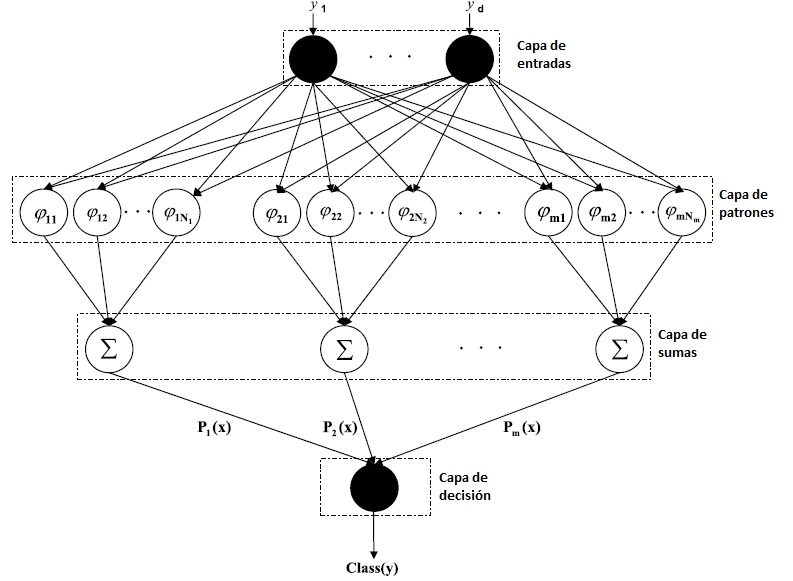
\includegraphics[scale=0.6]{Pic/RedPNN}
	\caption{Esquema de propagación hacia atrás.\cite{Art15}}
	\label{05}
	\hrule
\end{figure}

%%%%%%%%%%%%%%%%%%%%%%%%%%%%%%%%%%%%%%%%%%%%%%%%%%%%%%%%%%%%%%%%%%%%%%%%%%
\section{Problemas de clasificación}
En los problemas de clasificación se trata de determinar el tipo de categoría al que pertenece un elemento desconocido mediante técnicas de aprendizaje. Como ejemplo están los diagnósticos médicos o las predicciones de capacidad de pago de un crédito \cite{Guia17}. Se destacan algunas técnicas de Machine Learning utilizadas en problemas de clasificación.

\subsection{Técnicas de Machine Learning para Clasificación}
 \begin{itemize}
\item Regresión logística(logistic regression)
\item Máquinas de vectores de soporte(support vector machines)
\item Arboles de decisión(decision trees)
\item Bosques aleatorios(random forests)
\item Redes neuronales y aprendizaje profundo(deep learning)
\end{itemize}

%%%%%%%%%%%%%%%%%%%%%%%%%%%%%%%%%%%%%%%%%%%%%%%%%%%%%%%%%%%%%%%%%%%%%
%  ********************************
%     APLICACION DEL PROBLEMA ******%%%%%%%%%%%%%%%%%%%%%%%%%%%%%%%%%%%%%
%  ********************************
\chapter{Aplicación de Redes Neuronales a un problema de clasificación}
El objetivo de ANS es tratar de buscar modelos que solucionen problemas difíciles de resolver mediante técnicas algorítmicas convencionales. Por ejemplo, una aplicación del Chase Manhattan Bank para la concesión de préstamos, es un sistema mixto que incorpora herramientas estadísticas y un perceptrón multicapa \cite{Guia17}.

%%%%%%%%%%%%%%%%%%%%%%%%%%%%%%%%%%%%%%%%%%%%%%%%%%%%%%%%%%%%%%%%%%%%%%%%%%
\subsection{Aprobación de crédito}
La aprobación de un crédito es una decisión no estructurada\footnote{La decisión no estructurada es aquella que necesita de un modelo o proceso específico de solución \cite{Int08}}. con cierto riesgo del incumplimiento de pago por parte de los prestatarios que toman los analistas de crédito. Por tanto, las solicitudes de créditos deben ser evaluadas en un modelo de decisión, por parte de los analistas de crédito en las entidades crediticias, considerando algunos criterios e indicadores como radios de liquidez, rentabilidad, endeudamiento, las tasas de interés, plazos de tiempo, comisiones, historial, récord, garantía, capacidad de pago, endeudamiento, capital, las obligaciones, el compromiso, y la confianza en las personas.\\

La evaluación del riesgo crediticio de cada modalidad de crédito o contrato se realizará de acuerdo con una metodología que fije el respectivo organismo de dirección de la entidad vigilada, atendiendo para ello los parámetros mínimos establecidos. Un proceso particular de la evaluación del riesgo es la fragmentación de cartera, donde se puede clasificar las solicitudes de crédito según los indicadores mencionados anteriormente, mediante variables financieras.Ciertamente, existe una relación de las variables financieras que esta asociada un problemas de clasificación, y define una variable categórica(cualitativa) como respuesta(salida) al solicitante del crédito. De la misma manera, permite realizar predicciones de algunas variables numéricas(cuantitativa) que influyen en la toma de decisión. 

%%%%%%%%%%%%%%%%%%%%%%%%%%%%%%%%%%%%%%%%%%%%%%%%%%%%%%%%%%%%%%%%%%%%%%%%%%
\section{Modelar un problema de clasificación}
Las redes neuronales suelen ser utilizadas como herramientas para la predicción de tendencias y como clasificadoras de conjuntos de datos.
La aplicación de ANS a la predicción de un problema de clasificación se relaciona mediante las siguientes etapas, que se describen a continuación:

%%%%%%%%%%%%%%%%%%%%%%%%%%%%%%%%%%%%%%%%%%%%%%%%%%%%%%%%%%%%%%%%%%%%%%%%%%
\subsection{Recopilación de los datos} \label{DB}
Se encarga de detectar los orígenes de los datos para lograr conseguir de la forma más automatizada de captura, para su posterior análisis exploratorio \cite{Tes18}.\\
En la base de datos UC Irvine Machine Learning Repository \ref{07}, se presenta un problema de clasificación donde las definiciones de las variables no se suministran por motivos de confidencialidad \cite{Rev19}.

\subsection{Búsqueda de las variables de entrada}
Tiene como objetivo identificar las variables independientes que se relacionan con la variable dependiente a predecir, y se consideran entradas de la red.\\ Las variables se clasifican de la forma siguiente: 
\subsubsection{Variables independientes:} 
\begin{description}
	\item[Categórica] A1, A4, A5, A6, A7, A9, A10, A12, A13. 
	\item[Numérica] A2, A3, A8, A14, A11, A15.
\end{description} 

\subsubsection{Variable dependiente:} 
\begin{description}
	\item[Categórica] A16(Aprobación de crédito).
\end{description}   

\subsection{Análisis exploratorio}
Es el tratamiento estadístico al que se someten las muestras recogidas durante un proceso de investigación en cualquier campo científico( John W. Tukey) \cite{Int08}. El proceso de describe en las etapas siguientes:

\begin{enumerate}
	\item Preparación preliminar de los datos.
	\item Validación y depuración de los datos, se examinan los datos con el propósito de validar.
	\item Normalización o escalamiento de los datos, de ser necesario.
	\item Elección de técnica de análisis(ANS).
\end{enumerate}

La técnica ANS de inteligencia artificial, es uno de los instrumentos de uso frecuente para detectar categorías comunes en los datos, ya que son capaces de detectar y aprender patrones, y características de los datos. 

\subsection{Creación de la red}
PNN es a menudo utilizado en problemas de clasificación \cite{Int08}. Por lo tanto, se considera su arquitectura de red en el conjunto de datos para predecir la aprobación de crédito, y basado en el proceso de la sección \ref{08}, se definen los elementos siguientes:
\begin{description}
	\item[1. Entradas y salidas:] 15 variables independientes como entradas y 1 variable dependiente como salida.
	
	\item[2. Nodos ocultos:] Una capa oculta de 690 nodos(un nodo por cada caso) y otra de 2 nodos(categorias de la variable dependiente).  
	
	\item[3. Función de red:] Regla de clasificación bayesiana. 
	
	\item[4. Función de activación:] $ \varphi_{jk} = \dfrac{1}{(\sqrt{2\pi}\sigma)^d} \exp{(-\dfrac{1}{2\sigma^2})(x-{m_{jk}}^x)^2} $
	Ver en la sección \ref{10}
	\item[5. Interconexión entre nodos:] Unidireccional.
	\item[6. Propagación de red:] Hacia adelante. 
	\item[7. Selección de datos:] Datos del problema aprobación de crédito.
\end{description}

\subsection{Entrenamiento}
Se define el algoritmo de aprendizaje y sus parámetros de configuración. En esta aplicación un software considera las redes mas comunes en problemas de clasificación, para elegir el algoritmo de entrenamiento mas preciso. 

\subsection{Validación}
En esta etapa se realiza la validación del proceso de aprendizaje. Luego de presentar a la red el conjunto de datos seleccionados se obtienen los valores del siguiente periodo mediante los factores de comparación \cite{Art01}.

\subsubsection{Calcular factores de comparación}
Consiste en calcular los factores que serán utilizados en el análisis de los resultados al comparar los distintos modelos de redes neuronales obtenidos. Para realizar esta etapa, se obtienen los factores siguientes: 
\begin{itemize}
	\item Tiempo de Entrenamiento
    \item Número de pruebas
	\item Porcentaje de predicciones incorrectas
	\item Probabilidad incorrecta media
	\item Desviación estándar de probabilidad incorrecta
\end{itemize}
% *********************************************
% *********************************************
%%%%%%%%%%%%%%%%%%%%%%%%%%%%%%%%%%%%%%%%%%%%%%%%%%%%%%%%%%%%%%%%%%%%%%%%%%
\section{Software} \label{SF}
NeuralTools es un programa auxiliar de redes neuronales complementario de Microsoft Excel que permite analizar datos(incluso incompletos) en las hojas de cálculo de Excel y trabajar en el entorno familiar de Microsoft Office. Combinando un eficaz administrador de datos para el análisis exploratorio y la incorporación de los más modernos algoritmos de ANS para hacer las mejores predicciones tanto en problemas de clasificación(predicción de categoría) como en problemas numéricos. Ademas, incluye predicción en vivo, que permite predecir valores cuando se introducen nuevos datos en la hoja de cálculo de Excel. Estos cálculos se producen automáticamente.\\

NeuralTool se utiliza para desarrollar redes neuronales en cuatro pasos: \cite{Guia17}
\begin{description}

\item[Preparación de datos] Se definen en conjuntos de datos. El Administrador de
conjunto de datos se usa para configurar los conjuntos de datos.

\item[Entrenamiento] Con el entrenamiento se genera una red neuronal a partir de un conjunto de datos compuesto de casos con valores de salida conocidos. 

\item[Prueba] Se comprueba la red neuronal para ver cómo realiza la predicción de los valores de salida conocidos. Después de la prueba, se mide el funcionamiento de la red mediante estadísticos.

\item[Predicción] Se usa una red neuronal entrenada para predecir valores de salida  de casos nuevos.
\end{description}

% *********************************************
\chapter{Análisis de datos} 

En el análisis de la base de datos descrita en la Sección \ref{DB}, se determina como factor principal el nivel de medición de las variables. El conjunto de datos contiene 690 decisiones de aprobar o denegar un crédito, basándose en 15 variables(categóricas y numéricas) independientes.  En algunos casos faltan datos y el software ignorará estos casos. Los 3 primeros casos representan nuevos solicitantes de préstamo y se desconocen las decisiones de crédito para ellos. La ejecución del entrenamiento se realizo bajo las condiciones \textit{Probar automáticamente}, \textit{Predecir automáticamente} y \textit{Calcular impacto de variables}. Se utilizó la opción \textit{Búsqueda de mejor red} de la configuración de red. En la pestaña Tiempo de ejecución, se activó la casilla \textit{Pruebas} para acelerar la búsqueda de objetivos del problema. 

\section{Selección de Red}
Para encontrar el modelo más eficiente el software descrito en la Sección \ref{SF}, utiliza las redes MLFN(Perceptrón multicapa) de 2 a 6 nodos y PNN(Red probabilística) para modelar el problema y buscar la red con el mínimo error. En la tabla \ref{23} se muestran los resultados,  determinando que la red seleccionada es PNN.

\begin{figure}[h] \centering
\begin{tabular}{| m{4cm} | m{3cm} | m{5cm} |} \hline
\multicolumn{3}{|c|}{\textbf{Búsqueda de mejor red} }\\ \hline
\textbf{Tipo de red} &	\%\textbf{Error} &	\textbf{Tiempo de Entrenamiento}\\ \hline
PNN	        &    9.23\%	& 0:00:13\\ \hline
MLFN 2 nodos&	10.77\%	& 0:00:07\\ \hline
MLFN 3 nodos&	13.08\%	& 0:00:10\\ \hline
MLFN 4 nodos&	10.77\%	& 0:00:14\\ \hline
MLFN 5 nodos&	11.54\%	& 0:00:16\\ \hline
MLFN 6 nodos&	12.31\%	& 0:00:20\\ \hline
\end{tabular}
\caption{Tabla de resultados de la búsqueda de mejor red. [Fuente: propia]\label{23}}
\hrule 
\end{figure}

% ********************************************
% ********************************************
\section{Relación y predicción de variables}
Con el entrenamiento se genera una PNN a partir de un conjunto de datos compuesto de casos con valores de salida conocidos. Posteriormente, se aplica a los nuevos casos de los que no se conocen los valores de salida y se quieren clasificar mediante el proceso de validación.\\

La PNN utiliza reglas de clasificación bayesiana para encontrar la relación entre las variables y predecir valores desconocidos de una variable categórica. A continuación, en la tabla \ref{21} se muestran algunas predicciones calculadas mediante el Software descrito en la Sección \ref{SF}, para algunos casos seleccionados aleatoriamente de entrenamiento(95\% son correctos), prueba(90\% son correctos) y los tres casos de predicción.\\

\begin{figure}[h] \centering
\begin{tabular}{| m{2cm} | m{2cm} | m{2.3cm} |m{2.3cm} | m{2.5cm} |} \hline
\multicolumn{5}{|c|}{\textbf{Informe de entrenamiento Prueba-Predicción} }\\ \hline
\textbf{Etiqueta} &	\textbf{Aprobación} & \%\textbf{Predicción} &	\%\textbf{Incorrecto}   & \textbf{Correcto/Inc.}\\ \hline
predecir&	Sí&	53.40\% & &\\ \hline		
predecir&	Sí&	98.38\% & &\\ \hline		
predecir&	Sí&	87.50\% & &\\ \hline		
probar&	Sí    &	91.29\% &	8.71\%	&Correcto\\ \hline
entrenar&     &			& &\\ \hline
probar&	Sí    &	100.00\%&	0.00\%&	Correcto\\ \hline
entrenar&     &			&  &\\ \hline
probar&	No    &	74.71\% &74.71\% &	Incorrecto\\ \hline
\end{tabular}
\caption{Tabla de resultado de algunas predicciones del entrenamiento. [Fuente: propia]\label{21}}
\hrule
\end{figure}  
%%%%%%%%%%%%%%%%%%%%%%%%%%%%%%%%%%%%%%%%%%%%%%%%%%%%%%%
El entrenamiento de la red PNN, da como resultado la clasificación de aprobación de solicitudes de créditos, los cuales se resumen en las tablas \ref{22}, en una comparación de los valores reales vs las predicciones del entrenamiento y las pruebas.

\begin{figure}[h]
\centering
\subfloat{
\begin{tabular}{| m{3cm} | m{2.5cm} | m{2.5cm} | m{2.5cm} |}\hline
	\multicolumn{4}{|c|}{\textbf{Clasificación real vs predicción de entrenamiento}}\\ \hline
	\textbf{Clasificación}	& No(predicción)	& Sí(predicción) &    \%\textbf{Incorrecto}\\ \hline
	\textbf{No}(real)	& 273&13 &	4.5455\% \\ \hline
	\textbf{Sí}(real)	& 12	& 222 &	5.1282\% \\ \hline
\end{tabular}}
\caption{Tabla de matriz de clasificación de entrenamiento.}
\hrule
\subfloat{
\begin{tabular}{| m{3cm} | m{2.5cm} | m{2.5cm} | m{2.5cm} |}\hline
	\multicolumn{4}{|c|}{\textbf{Clasificación real vs predicción de pruebas}}\\ \hline
	\textbf{Clasificación}	& No(predicción)	& Sí(predicción) &    \%\textbf{Incorrecto}\\ \hline
	\textbf{No}(real)	& 64&7 &	9.8592\% \\ \hline
	\textbf{Sí}(real)	& 5	& 54 &	8.4746\% \\ \hline
\end{tabular}}
\caption{Tabla de matriz de clasificación de valores de pruebas.[Fuente: propia]\label{22}}
\hrule
\end{figure} 
%%%%%%%%%%%%%%%%%%%%%%%%%%%%%%%%%%%%%%%%%%%%%%%%%%%%%%%%5
También se muestra el gráfico \ref{23}, para ilustrar que la variable $A8$ es el factor más importante de estas predicciones.\\
\begin{figure}[h]
	\centering
	\subfloat{
		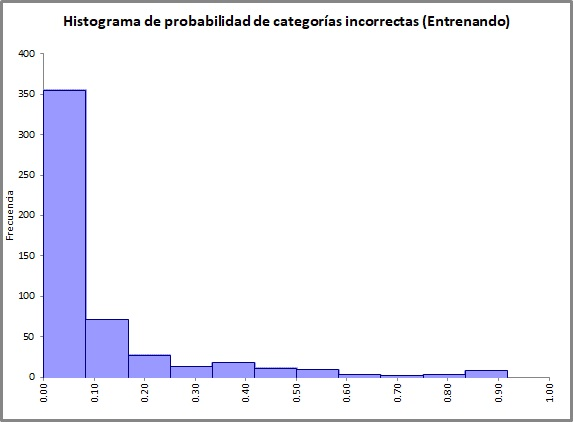
\includegraphics[scale=0.5]{Pic/HistogramaEntren}}
	\caption{Histograma de probabilidad de categorías incorrectas de entrenamiento.\label{23}}
	\subfloat{
		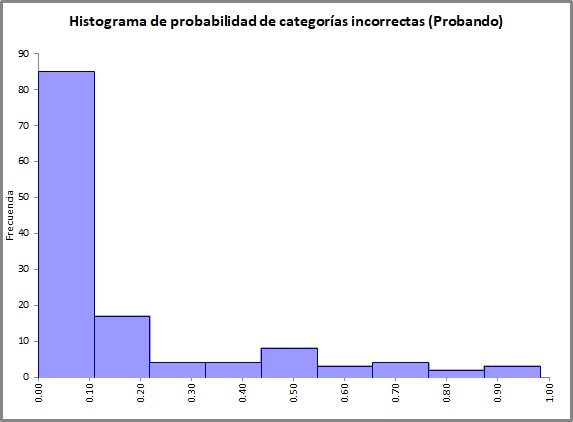
\includegraphics[scale=0.5]{Pic/HistogramaPrueba}}
	\caption{Histograma de probabilidad de categorías incorrectas de pruebas.[Fuente: propia]\label{23}}
\end{figure}


% ********************************************
\section{Análisis de Resultados}
El informe de resumen de entrenamiento ofrece estadísticas y gráficos sobre
el funcionamiento de la red PNN entrenada. En la Figura \ref{22}, se presentan los resultados mas importantes del informe generado por la entrenamiento. La validación de la red, se realiza mediante la interpretación de los resultados objetivos del entrenamiento, entre los cuales se consideran las de predicciones incorrectas que representan el porcentaje de casos para los que la categoría de la predicción no coincide con la categoría real. De la misma manera, se considera la Probabilidad incorrecta media como la probabilidad promedio de categorías incorrectas.

\begin{figure}[h]
	\centering
		\begin{tabular}{| m{7cm} | m{3cm} | m{2cm} |}\hline
\textbf{Resultados de la aplicación PNN} & \textbf{Entrenamiento} & \textbf{Pruebas}\\ \hline
Número de casos	& 520 &	130 \\ \hline
\% predicciones incorrectas &	4.8\% &	9.2\%\\ \hline
Probabilidad incorrecta media &	10.9\% &	15.8\%\\ \hline
Desviación estándar de prob. incorrecta &	17.1\% &	23.4\% \\ \hline
	\end{tabular}
	\caption{Tabla de resultados de la aplicación PNN. [Fuente: propia]\label{22}}
	\hrule
\end{figure} 

%%%%%%%%%%%%%%%%%%%%%%%%%%%%%%%%%%%%%%%%%%%%%%%%%%%%%%%%%%%%%%%%%%
\chapter{Conclusiones}
La teoría sobre la funcionalidad de las redes neuronales artificiales se basa en el sistema neuronal biológico para modelar problemas de la vida real utilizando técnicas de aprendizaje.\\

Cada día las redes neuronales artificiales se vuelven mas importantes por su diversidad de aplicaciones lineales y no lineales en los diferentes campos de estudio, ya que han generado soluciones muy confiables a los problemas.\\

La estructura de las redes neuronales artificiales permite utilizar otras técnicas para obtener buenos resultados. Sin embargo, no es posible considerar a una técnica de aprendizaje mejor que otra, ya que su eficiencia depende del área de aplicación y del resultado esperado.\\

Las redes neuronales artificiales han sido utilizadas durante mucho tiempo para modelar problemas de clasificación ya que son capaces de detectar y aprender patrones de los datos.\\  

No hay ningún criterio establecido para decidir la arquitectura final de una red neuronal, el número de capas y el número de neuronas de cada una de estas es fijado por la experiencia del diseñador o mediante el ensayo diferentes tipos de red comparando el error.\\

En la aplicación del problema aprobación de crédito, se selecciona la red probabilística porque tiene el mínimo error 9.23\%. Esta red utiliza reglas de clasificación bayesiana para predecir y a calcula la probabilidad de que la predicción sea de otra categoría. Los resultados de la red seleccionada tienen un 4.8\% de predicciones incorrectas en el entrenamiento y un 9.2\% en las pruebas.


% ********************************************
% ********************************************



\newpage
\bibliographystyle{amsplain}
\begin{thebibliography}{12}
	
\bibitem[1]{Art01}Luis Escobar R, Julio Valdes H y Santiago Zapata C, \textit{Redes Neuronales Artificiales en predicción de Series de Tiempo}, Universidad de Palermo, Argentina.
	
\bibitem[2]{Art02}Xabier Basogain Olabe, \textit{Redes Neuronales Artificiales y sus Aplicaciones}, Escuela Superior de Ingeniería de Bilbao, España.

 \bibitem[3]{Lib03}Requena y Ignacio, \textit{Introducción a las Redes Neuronales Artificiales. Neurocomputación}, Universidad de Granada, España.

\bibitem[4]{Lib04}Correa y Rafael(2006), \textit{Redes Neuronales Artificiales en Ingeniería y Física Nuclear. Caracterización de espectros PIXE}, Universidad de Granada, España.

\bibitem[5]{Lib05}Zhang y Peter(2004), \textit{Neural Networks in Business Forecasting}, 1 edición, Idea Group Publishing, E.U.A.

\bibitem[6]{Lib06}James Freeman y David Skapura(1993), \textit{Redes Neuronales Algoritmos, aplicaciones y técnicas de programación}, 1 edición, Addison-Wesley Iberoamericana, E.U.A.


\bibitem[7]{Art07}John Villavicencio, \textit{Introducción a Series de Tiempo.}

\bibitem[8]{Int08}https://es.wikipedia.org/wiki, Aprendizaje por refuerzo.

\bibitem[9]{Int09}http://labcienciasnestor.blogspot.com/2010/05/generalidades-de-las-neurona.html, Generalidades de las Neurona.

\bibitem[10]{Int10}https://www.researchgate.net/figure/La-neurona-biologicafig1750837616, Diseño y experimentación de un cuantizador vectorial.
 
\bibitem[11]{Int11}http://www.cs.us.es/~fsancho/?e=72, Modelo neuronal de McCulloch-Pitts.
  
\bibitem[12]{Lib12}2005, \textit{Artificial neuronal networks in Intensive Medicine. An example of application with MPM II variables}.

\bibitem[13]{Art13}Huayna, Ana M., Calvo, Vanessa H., Huiman, Juan C.(2010), \textit{Modelo de Evaluación de Créditos Financieros basados en Redes Neuronales orientado a Edpymes}, Universidad Nacional Mayor de San Marcos, Perú.

\bibitem[14]{Art14}Berzal, Fernando(2015), \textit{Redes Neuronales}, Psychological Science, 2nd edition, W.W. Norton and Company, Universidad de Granada, España.

\bibitem[15]{Art15}Gutiérrez, Paloma T., Vázquez, José A.(2013), \textit{Aplicación de la Red Neuronal Probabilística para la clasificación
	de productos conforme a sus especificaciones.}, Instituto Tecnológico de Celaya, Celaya, Guanajuato, México.

\bibitem[16]{Art16}Ramírez Q. Juan A., Chacón M. Mario I.(2011) \textit{Redes neuronales artificiales para el procesamiento de imágenes, una revisión de la última década}, Revista de ingeniera eléctrica, México.

\bibitem[17]{Guia17}\textit{Guía para el uso de NeuralTools}, Palisade Corporation, Ithaca, NY, E.U.A.

\bibitem[18]{Tes18}Moreno E., Gimena A.(2008), \textit{Diseño de un modelo para Agentes basados en Redes Neuronales para WebMining.}, Tesis de grado de Ingeniero en Sistemas Informáticos y Computación, La Universidad Católica de Loja, Ecuador.

\bibitem[19]{Rev19}Del Carpio Gallegos, Javier(2005), \textit{Redes Neuronales en el campo de las finanzas}, vol. 8,  Industrial Data, Universidad Nacional Mayor de San Marcos, Perú.

\bibitem[20]{DB20} \label{07}http://archive.ics.uci.edu/ml/datasets/Credit+Approval, \textit{UC Irvine Machine Learning Repository}.
\end{thebibliography}

% ********************************************%%%%%%%%%%%%%%%%%%%%
% ********************************************

\chapter{Anexos}


\section{Resumen base de datos bibliográfica.}

\begin{tabular}{ |p{3cm} | p{9cm} | p{2cm} |} 	\hline
	\begin{center}
		
\includegraphics[width=1.2cm]{Pic/UNAH}
	\end{center} 	& 
	\begin{center}
		\textbf{ESTADO DEL ARTE: UN BREVE ESTUDIO DE REDES NEURONALES.}
	\end{center}       	& 
	\begin{center}
		
\includegraphics[width=1.5cm]{Pic/Facu_ciencias.jpg} 
	\end{center}  	\\ \hline \hline
	% primera fila ##############################################
	
	\textbf{ Base de datos}   & \textbf{Titulo}    & \textbf{Archivo}    \\ \hline
	
	Biblioteca UNAH   & Neural Networks. Algorithms, Aplications, and Programming Techniques & Libro \\ \hline
	
	Google Académico & Redes Neuronales Artificiales en predicción de Series de Tiempo & Articulo \\ \hline
	
	Dialnet & Introducción a las Redes Neuronales Artificiales. Neurocomputación & Libro \\ \hline
	
	
	Open Access Theses and Dissertations & Redes Neuronales Artificiales en Ingeniería y Física Nuclear. Caracterización de espectros PIXE & Libro \\
	
	ResearchGate   &   Neural Networks in Business Forecasting    &  Articulo \\ \hline
	
	Google académico  &  Introducción a Series de Tiempo    &   \\ \hline
	\end{tabular} 
% ********************************************%%%%%%%%%%%%%%%%%%%%%%%%%%%%%%%%%%%%%%%
% ******************************************** FIN BASE DE DATOS BIBLIOGR. %%%%%%%%%%
\clearpage
\section{Ficha descriptiva Lib-01}
\begin{table}[h]
\centering
\begin{tabular}{|>{\centering\arraybackslash}m{3cm}|m{9cm}|>{\centering\arraybackslash}m{3cm}|} 	\hline
  
\vspace{0.4cm} 
\includegraphics[width=1cm]{Pic/UNAH}  &  \textbf{UN BREVE ESTUDIO DE REDES NEURONALES.} 	& 
\includegraphics[width=1cm]{Pic/Facu_ciencias.jpg} \\ \hline \hline
% primera fila ##############################################

 \multicolumn{2}{|c|}{\textbf{FICHA DESCRIPTIVA}} & FICHA No.01  \\ \hline \textbf{Título Original}  & \multicolumn{2}{c|}{Redes Neuronales Artificiales en Predicción  de series de Tiempo. }\\ \hline 

\textbf{Autor(a)}  & \multicolumn{2}{c|}{Luis Escobar R, Julio Valdes H y Santiago Zapata C.{\LARGE . } }\\ \hline 

\multicolumn{3}{|c|}{ \textbf{2. Aspectos Formales} } \\ \hline
1.1 Tipo de autor   &   \multicolumn{2}{c|  }{\begin{tabular}{ m{1.8cm} |  m{0.7cm}  | m{1.8cm} | m{0.7cm}   | m{1.8cm} | m{0.7cm} } Colectivo  &  \makebox[1cm][c]{ X } &   Individual  &    & Institucional &   
\end{tabular}} \\ \hline

1.2 Tipo de Documento &  \multicolumn{2}{c| }{\begin{tabular}{m{1.8cm} |  m{0.7cm}  | m{1.8cm} | m{0.7cm}   | m{1.8cm} | m{0.7cm} } Libro  &   &   Articulo  &  \makebox[1cm][c]{ X }  & Tesis &   
\end{tabular}} \\ \hline

\textbf{2.1 Tema }  & \multicolumn{2}{c|}{Redes Neuronales Artificiales{\LARGE . } }\\ \hline 

\textbf{2.2 Núcleos temáticos}  & \multicolumn{2}{l|}{\begin{tabular}{p{12cm}}
	\begin{itemize}
		\item Funcionalidad de redes neuronales.
		\item Predicción de series de tiempo.
	\end{itemize} \end{tabular} }\\ \hline 

\textbf{2.3 Problemas propuestos}  & \multicolumn{2}{l|}{\begin{tabular}{p{12cm}}
	
		\begin{itemize}
			\item ¿ Cuales son los fundamentos de la teoría de una red neuronal?
			\item ¿Se puede modelar series de tiempo por medio de redes neuronales?
			\item  ¿ Las redes neuronales son mas precisas que otros métodos?
		\end{itemize}
\end{tabular}} \\ \hline
%%%
\end{tabular}
\end{table}

\begin{table}[ht!]
\centering	
\begin{tabular}{|>{\centering \arraybackslash}m{3cm}|m{8cm}|>{\centering \arraybackslash}m{3cm}|} 	\hline

\multicolumn{3}{|c|}{ \textbf{3. Delimitación contextual} } \\ \hline

\textbf{3.1 Espacial}  & \multicolumn{2}{c|}{Funcionalidad básica para predecir series temporales}\\ \hline 

\textbf{3.2 Temporal}  & \multicolumn{2}{c|}{El colectivo investigador no establece una delimitación temporal{\LARGE . } }\\ \hline 

\textbf{3.3 Sujetos investigados}  & \multicolumn{2}{l|}{\begin{tabular}{p{12cm}}
		\begin{itemize}
			\item Fundamentos básicos de la teoría de Redes Neuronales.
			\item Modelos de series temporales de generación de electricidad y consumo de gas.
			\item Alcance de las Redes Neuronales para predecir series temporales.
\end{itemize} \end{tabular} }\\ \hline 


\multicolumn{3}{|c|}{\textbf{4. Propósito } }         \\ \hline
\textbf{4.1 Objetivo General} & \multicolumn{2}{l|}{ \begin{tabular}{p{9cm}}
		Introducción a la teoría de funcionamiento y arquitectura de red neuronal.  
\end{tabular} } \\ \hline
\textbf{4.2 Objetivos Específicos} & \multicolumn{2}{l|}{ \begin{tabular}{p{9cm}}
		\begin{itemize}
			\item Una solida comprensión del funcionamiento de la red neuronal.
			
			\item  La capacidad de predecir series temporales.
			
			\item Comparar con las técnicas tradicionales para predecir series temporales. 
			
			\item Resolver problemas con la técnica redes neuronales.
			
		\end{itemize} 
\end{tabular} } \\ \hline
% finalizar tabla
\end{tabular}
\end{table}

\begin{table}[ht!]
	\centering
\begin{tabular}{|>{\centering\arraybackslash}m{3cm}|m{5cm}| m{5cm}|} 	\hline
\multicolumn{3}{|c|}{ \textbf{5. Enfoque} }             \\ \hline
\multicolumn{2}{|c|}{\textbf{5.1 S\'intesis} }     & \textbf{ Palabras Clave}    \\ \hline
\multicolumn{2}{|c|}{   \begin{tabular}{p{9cm}}
		
En esta investigación se han utilizado las redes neuronales artificiales en la predicción de dos series de tiempo tomadas del campo de la industria: Generación de Electricidad Mensual y Consumo Mensual de Gas Natural. Como parte del objetivo general de esta investigación se ha evaluado la capacidad que tienen las redes neuronales artificiales en la predicción de series de tiempo, resultando efectivas en esta tarea y demostrando que son una herramienta útil en la predicción de series de tiempo.

		
		
\end{tabular}  }    & \begin{tabular}{p{4cm}}
	\begin{itemize}
		\item Arquitectura de red
		\item Predicciones
		\item Aplicaciones
		\item Técnicas de análisis
		\item Algoritmos
		\item Propagación
		
	\end{itemize}
\end{tabular}  
\\ \hline

\multicolumn{3}{|c|}{ \textbf{6. Referencias} }             \\ \hline
\multicolumn{2}{|c|}{\textbf{6.1 Referencias Teóricas} }     & \textbf{Conceptos principales}    \\ \hline
\multicolumn{2}{|c|}{   \begin{tabular}{p{8cm}}
		
\begin{description}
	
	\bibitem[1] Kunihiko Fukushima, \textit{A self organizing multilayered neuronal network}, Biological Cybernetics, 1975.
	
	\bibitem[2] Robert Hecht Nielsen, \textit{ANZA User's Guide}, San Diego, USA, 1987.
		
	\bibitem[3] Murali Menon y Karl Heinemann, \textit{Clasification of patterns using a self organizing neural network}, 1988.
	
	
\end{description}
		
\end{tabular}  }    & \begin{tabular}{p{4.65cm}}
	\begin{itemize}
		\item El Sistema neuronal Biológico
		\item Perceptrón multicapa.
		\item Programación de la redes. 
		\item Aplicaciónes de Redes Neuronales a algunos problemas reales
	\end{itemize}
\end{tabular}  
\\ \hline
\end{tabular} 
\end{table}


\pagebreak
\begin{table}[ht!]
\centering
\begin{tabular}{| m{3cm} | m{8cm} | m{6cm} |} 	\hline
	\multicolumn{3}{|c|}{\textbf{7. Investigación} }         \\ \hline
7.1 Tipo de investigación   &   \multicolumn{2}{c|  }{\begin{tabular}{ m{2cm} |  m{0.7cm}  | m{2cm} | m{0.7cm}   | m{2cm} | m{0.7cm} } Exploratoria  & \makebox[1cm][c]{ X }  &   Descriptiva  &    & Explicativa &  \end{tabular}} \\ \hline


	\multicolumn{3}{|c|}{\textbf{8. Procedimiento} }         \\ \hline
8.1 Tipo de metodología   &   \multicolumn{2}{c|}{\begin{tabular}{ m{2cm} |  m{0.7cm}  | m{2cm} | m{0.7cm}   | m{2cm} | m{0.7cm} } Cualitativa  &   &   Cuantitativa  &  \makebox[1cm][c]{X} & Mixta &    \end{tabular}} \\ \hline

 \multicolumn{2}{|c|}{\textbf{8.2 Técnicas} }     & \textbf{Intención}    \\ \hline
 \multicolumn{2}{|c|}{   \begin{tabular}{p{6cm}}
 		
 		\begin{description}
 			
 			\item Perceptrón.
 			
 			\item Propagación hacia atrás.
 			
 			\item ARIMA.
 			
 			\item Regresíon lineal
 			
 			\item Propagación de la red
 			
 			\item Tramas de espacios temporales
 			
 			\item La predicción
 			
 		\end{description}
 		
 \end{tabular}  }    & \begin{tabular}{p{6cm}}
 	\begin{itemize}
 		\item Utilizar esta técnicas para modelar problemas. 
 		\item Encontrar patrones en los datos.
 		\item Conocer los fundamentos teóricos de una Red Neuronal. 
 		\item Comprender su funcionalidad para predecir series de tiempo.
 	\end{itemize}
 \end{tabular}  
 \\ \hline
\end{tabular} 
\caption{edes Neuronales Artificiales en predicción
	de Series de Tiempo. Una aplicación a la Industria.}
\end{table}


% ********************************************
% **********************************%%%%%%%%%%%%%%%%%%%%%%%%%%%%%%%%%%%%%%%%%%%%%%%
\clearpage
\section{Ficha descriptiva Art-02}
\begin{table}[ht!]
\centering	
\begin{tabular}{|>{\centering\arraybackslash}m{3cm}|m{9cm}|>{\arraybackslash}m{3cm}|} 	\hline
\vspace{0.4cm} 
\includegraphics[width=1cm]{Pic/UNAH}  &  \textbf{UN BREVE ESTUDIO DE REDES NEURONALES} 	& 
\includegraphics[width=1cm]{Pic/Facu_ciencias.jpg} \\ \hline \hline
% primera fila ##############################################
		
\multicolumn{2}{|c|}{\textbf{FICHA DESCRIPTIVA}} & FICHA No Art-02  \\ \hline \textbf{Título Original}  & \multicolumn{2}{c|}{Neural Networks. Algorithms, Aplications, and Programming Techniques{\LARGE . } }\\ \hline 
		
		\textbf{Título}  & \multicolumn{2}{c|}{Redes neuronales. Algoritmos, aplicaciones y técnicas de programación{\LARGE .} }\\ \hline 
		
		\textbf{Autor(a)}  & \multicolumn{2}{c|}{James A. Freeman y David M. Skapura{\LARGE . } }\\ \hline 
		
		\multicolumn{3}{|c|}{ \textbf{2. Aspectos Formales} } \\ \hline
		1.1 Tipo de autor   &   \multicolumn{2}{c|  }{\begin{tabular}{ m{1.8cm} |  m{0.7cm}  | m{1.8cm} | m{0.7cm}   | m{1.8cm} | m{0.7cm} } Colectivo  &  \makebox[1cm][c]{ X } &   Individual  &    & Institucional &   
		\end{tabular}} \\ \hline
		
		1.2 Tipo de Documento &  \multicolumn{2}{c| }{\begin{tabular}{m{1.8cm} |  m{0.7cm}  | m{1.8cm} | m{0.7cm}   | m{1.8cm} | m{0.7cm} } Libro  &  \makebox[1cm][c]{ X } &   Articulo  &    & Tesis &   
		\end{tabular}} \\ \hline
		
		\textbf{2.1 Tema central}  & \multicolumn{2}{c|}{Una introducción solida y practica a las Redes Neuronales{\LARGE . } }\\ \hline 
		
		\textbf{2.2 Núcleos temáticos}  & \multicolumn{2}{l|}{\begin{tabular}{p{12cm}}
				\begin{itemize}
					\item Arquitectura de una red neuronal.
					\item Teoria del funcionamiento de una red neuronal.
					\item Aplicaciones y algoritmos de Redes Neuronales.
		\end{itemize} \end{tabular} }\\ \hline 
		
		\textbf{2.3 Problemas propuestos}  & \multicolumn{2}{l|}{\begin{tabular}{p{12cm}}
				
				\begin{itemize}
					\item ¿ Cuales son los fundamentos de la teoría actual y del conocimiento de una red neuronal?
					\item ¿Que problemas se pueden modelar por medio de redes neuronales y cual es su alcance?
					\item  ¿Como esta compuesto un sistema de red neuronal?
				\end{itemize}
		\end{tabular}} \\ \hline
		%%%
	\end{tabular}
\end{table}

\begin{table}[ht!]
	\centering	
	\begin{tabular}{|>{\centering\arraybackslash}m{3cm}|m{8cm}|>{\centering\arraybackslash}m{3cm}|} 	\hline
		
		\multicolumn{3}{|c|}{ \textbf{3. Delimitación contextual} } \\ \hline
		
		\textbf{3.1 Espacial}  & \multicolumn{2}{c|}{El colectivo investigador no establece una delimitación espacial{\LARGE . } }\\ \hline 
		
		\textbf{3.2 Temporal}  & \multicolumn{2}{c|}{El colectivo investigador no establece una delimitación temporal{\LARGE . } }\\ \hline 
		
		\textbf{3.3 Sujetos investigados}  & \multicolumn{2}{l|}{\begin{tabular}{p{12cm}}
				\begin{itemize}
					\item Fundamentos teóricos Redes Neuronales.
					\item Modelos mas comunes de Redes Neuronales.
					\item Alcance de las Redes Neuronales.
		\end{itemize} \end{tabular} }\\ \hline 
		
		
		\multicolumn{3}{|c|}{\textbf{4. Propósito } }         \\ \hline
		\textbf{4.1 Objetivo General} & \multicolumn{2}{l|}{ \begin{tabular}{p{9cm}}
				Descripción general de la teoría de funcionamiento y arquitectura de la red neuronal.  
		\end{tabular} } \\ \hline
		\textbf{4.2 Objetivos Específicos} & \multicolumn{2}{l|}{ \begin{tabular}{p{9cm}}
				\begin{itemize}
					\item Una solida comprensión del funcionamiento de la red neuronal.
					
					\item  La capacidad de programar con éxito la simulación de una red neuronal.
					
					\item Aplicar redes neuronales a problemas reales de ciencia e ingeniería. 
					
					\item Resolver problemas que han eludido otras aproximaciones.
					
				\end{itemize} 
		\end{tabular} } \\ \hline
		% finalizar tabla
	\end{tabular}
\end{table}

\begin{table}[ht!]
	\centering
	\begin{tabular}{|>{\centering\arraybackslash}m{3cm}|m{5cm}| m{5cm}|} 	\hline
		\multicolumn{3}{|c|}{ \textbf{5. Enfoque} }             \\ \hline
		\multicolumn{2}{|c|}{\textbf{5.1 S\'intesis} }     & \textbf{ Palabras Clave}    \\ \hline
		\multicolumn{2}{|c|}{   \begin{tabular}{p{9cm}}
				
				En este libro de texto se pretende satisfacer la continua necesidad de tener una visión general de la arquitectura de red neuronal y una descripción detallada de la teoría de funcionamiento de la red para que el lector aprenda a modelar problemas reales por medio de redes neuronales. De la misma manera, desarrollar algoritmos, aplicaciones y técnicas como la propagación hacia atrás para la programación y encontrar la resolución a estos problemas.
				
				
		\end{tabular}  }    & \begin{tabular}{p{4cm}}
			\begin{itemize}
				\item Arquitectura
				\item Resolución
				\item Aplicaciones
				\item Técnicas
				\item Algoritmos
				\item Propagación
				
			\end{itemize}
		\end{tabular}  
		\\ \hline
		
		\multicolumn{3}{|c|}{ \textbf{6. Referencias} }             \\ \hline
		\multicolumn{2}{|c|}{\textbf{6.1 Referencias Teóricas} }     & \textbf{Conceptos principales}    \\ \hline
		\multicolumn{2}{|c|}{   \begin{tabular}{p{8cm}}
				
				\begin{description}
					
					\bibitem[1] Kunihiko Fukushima, \textit{A self organizing multilayered neuronal network}, Biological Cybernetics, 1975.
					
					\bibitem[2] Robert Hecht Nielsen, \textit{ANZA User's Guide}, San Diego, USA, 1987.
					
					\bibitem[3] Murali Menon y Karl Heinemann, \textit{Clasification of patterns using a self organizing neural network}, 1988.
					
					
				\end{description}
				
		\end{tabular}  }    & \begin{tabular}{p{4.65cm}}
			\begin{itemize}
				\item El Sistema neuronal Biológico como modelo matemático
				\item Funcionamiento de algunas redes comunes.
				\item Programación de simulaciones de estas redes. 
				\item Aplicación de Redes Neuronales a algunos problemas reales
			\end{itemize}
		\end{tabular}  
		\\ \hline
	\end{tabular} 
	
	
\end{table}


\pagebreak
\begin{table}[ht!]
	\centering
	\begin{tabular}{| m{3cm} | m{8cm} | m{6cm} |} 	\hline
		\multicolumn{3}{|c|}{\textbf{7. Investigación} }         \\ \hline
		7.1 Tipo de investigación   &   \multicolumn{2}{c|  }{\begin{tabular}{ m{2cm} |  m{0.7cm}  | m{2cm} | m{0.7cm}   | m{2cm} | m{0.7cm} } Exploratoria  &   &   Descriptiva  &  \makebox[1cm][c]{ X }  & Explicativa &  \end{tabular}} \\ \hline
		
		
		\multicolumn{3}{|c|}{\textbf{8. Procedimiento} }         \\ \hline
		8.1 Tipo de metodología   &   \multicolumn{2}{c|}{\begin{tabular}{ m{2cm} |  m{0.7cm}  | m{2cm} | m{0.7cm}   | m{2cm} | m{0.7cm} } Cualitativa  &   &   Cuantitativa  &   & Mixta & \makebox[1cm][c]{X}   \end{tabular}} \\ \hline
		
		\multicolumn{2}{|c|}{\textbf{8.2 Técnicas} }     & \textbf{Intención}    \\ \hline
		\multicolumn{2}{|c|}{   \begin{tabular}{p{6cm}}
				
				\begin{itemize}
					
					\item Adeline y Madaline.
					
					\item Propagación hacia atrás.
					
					\item La BAM y la memoria de Hopfield.
					
					\item Temple simulado
					
					\item Red de contrapropagación
					
					\item Tramas de espacios temporales
					
					\item El neocognitrón
					
				\end{itemize}
				
		\end{tabular}  }    & \begin{tabular}{p{6cm}}
			\begin{itemize}
				\item Utilizar estas técnicas para modelar problemas. 
				\item Crear inteligencia artificial.
				\item Conocer los fundamentos teóricos y prácticos de una Red Neuronal. 
				\item Crear algoritmos para obtener una resolución al problema.
			\end{itemize}
		\end{tabular}  
		\\ \hline
	\end{tabular} 
	\caption{Redes Neuronales Artificiales en predicción de Series de Tiempo.}
\end{table}

%%%%%%%%%%%%%%%%%%%%%%%%%%%%%%%%%%%%%%%%%%%%%%%%%%%%%%%%%%%%%%%%

% **********************************%%%%%%%%%%%%%%%%%%%%%%%%%%%%%%%%%%%%%%%%%%%%%%%
\clearpage
\section{Ficha descriptiva Art-03}
\begin{table}[ht!]
	\centering	
	\begin{tabular}{|>{\centering\arraybackslash}m{3cm}|m{9cm}| m{3cm}|} 	\hline
		\vspace{0.4cm} 
\includegraphics[width=1cm]{Pic/UNAH}  &  \textbf{UN BREVE ESTUDIO DE REDES NEURONALES} 	& 
\includegraphics[width=1cm]{Pic/Facu_ciencias.jpg} \\ \hline \hline
		% primera fila ##############################################
		
		\multicolumn{2}{|c|}{\textbf{FICHA DESCRIPTIVA}} & FICHA No Art-03  \\ \hline \textbf{Título Original}  & \multicolumn{2}{c|}{Redes Neuronales y sus Aplicaciones}\\ \hline 
		
		\textbf{Autor(a)}  & \multicolumn{2}{c|}{Xabier Basogain Olabe}\\ \hline 
		
		\multicolumn{3}{|c|}{ \textbf{2. Aspectos Formales} } \\ \hline
		1.1 Tipo de autor   &   \multicolumn{2}{c|  }{\begin{tabular}{ m{1.8cm} |  m{0.7cm}  | m{1.8cm} | m{0.7cm}   | m{1.8cm} | m{0.7cm} } Colectivo  &  \makebox[1cm][c]{ X } &   Individual  &    & Institucional &   
		\end{tabular}} \\ \hline
		
		1.2 Tipo de Documento &  \multicolumn{2}{c| }{\begin{tabular}{m{1.8cm} |  m{0.7cm}  | m{1.8cm} | m{0.7cm}   | m{1.8cm} | m{0.7cm} } Libro  &  \makebox[1cm][c]{ X } &   Articulo  &    & Tesis &   
		\end{tabular}} \\ \hline
		
		\textbf{2.1 Tema central}  & \multicolumn{2}{c|}{Introducción a la computación neuronal}\\ \hline 
		
		\textbf{2.2 Núcleos temáticos}  & \multicolumn{2}{l|}{\begin{tabular}{p{12cm}}
				\begin{itemize}
					\item Características de una red neuronal.
					\item Estructura básica de una red neuronal.
					\item Computación tradicional y neuronales.
		\end{itemize} \end{tabular} }\\ \hline 
		
		\textbf{2.3 Problemas propuestos}  & \multicolumn{2}{l|}{\begin{tabular}{p{12cm}}
				
				\begin{itemize}
					\item ¿ Cuales son los fundamentos de la teoría  de la computación neuronal?
					\item ¿Que implementación y tecnologías emergentes surgen con redes neuronales?
					\end{itemize}
		\end{tabular}} \\ \hline
		%%%
	\end{tabular}
\end{table}

\begin{table}[ht!]
	\centering	
	\begin{tabular}{|>{\centering\arraybackslash}m{3cm}|m{8cm}|>{\centering\arraybackslash}m{3cm}|} 	\hline
		
		\multicolumn{3}{|c|}{ \textbf{3. Delimitación contextual} } \\ \hline
		
		\textbf{3.1 Espacial}  & \multicolumn{2}{c|}{Diseño de una red neuronal para una aplicación.}\\ \hline 
		
		\textbf{3.2 Temporal}  & \multicolumn{2}{c|}{El colectivo investigador no establece una delimitación temporal{\LARGE . } }\\ \hline 
		
		\textbf{3.3 Sujetos investigados}  & \multicolumn{2}{l|}{\begin{tabular}{p{12cm}}
				\begin{itemize}
					\item Características de Redes Neuronales.
					\item Estructura básica de Redes Neuronales.
					\item Computación tradicional y neuronal.
		\end{itemize} \end{tabular} }\\ \hline 
		
		
		\multicolumn{3}{|c|}{\textbf{4. Propósito } }         \\ \hline
		\textbf{4.1 Objetivo General} & \multicolumn{2}{l|}{ \begin{tabular}{p{9cm}}
				Descripción general de la teoría y diseño de la red neuronal para su aplicación.  
		\end{tabular} } \\ \hline
		\textbf{4.2 Objetivos Específicos} & \multicolumn{2}{l|}{ \begin{tabular}{p{9cm}}
		\begin{itemize}
					\item Una solida comprensión del funcionamiento de la red neuronal.
					
					\item  La capacidad de programar mediante computación neuronal.
					
					\item Implementación de tecnologías emergentes. 
		\end{itemize} 
		\end{tabular} } \\ \hline
		% finalizar tabla
	\end{tabular}
\end{table}

\begin{table}[ht!]
	\centering
	\begin{tabular}{|>{\centering\arraybackslash}m{3cm}|m{5cm}| m{5cm}|} 	\hline
		\multicolumn{3}{|c|}{ \textbf{5. Enfoque} }             \\ \hline
		\multicolumn{2}{|c|}{\textbf{5.1 S\'intesis} }     & \textbf{ Palabras Clave}    \\ \hline
		\multicolumn{2}{|c|}{   \begin{tabular}{p{9cm}}
				
En este articulo académico se pretende comprender la funcionalidad básica y la implementación de computación neuronal en una diversidad de aplicaciones de las redes neuronales y difusos.  De la misma manera, desarrollar algoritmos, aplicaciones y técnicas para implementación de tecnologías emergentes.
				
				
		\end{tabular}  }    & \begin{tabular}{p{4cm}}
		\begin{itemize}
				\item Computación neuronal
				\item Aplicaciones
				\item Técnicas
				\item Algoritmos
				\item Implementación
				\item Lógica difusa
		\end{itemize}
		\end{tabular}  
		\\ \hline
		
		\multicolumn{3}{|c|}{ \textbf{6. Referencias} }             \\ \hline
		\multicolumn{2}{|c|}{\textbf{6.1 Referencias Teóricas} }     & \textbf{Conceptos principales}    \\ \hline
		\multicolumn{2}{|c|}{   \begin{tabular}{p{8cm}}
				
				\begin{description}
					
					\bibitem[1] Pedro Isasi Viñuela , Inés M. Galván León, 2003, \textit{Redes de Neuronas Artificiales. Un enfoque Práctico}, Pearson Prentice Hall.
					
					\bibitem[2] Francisco J. Rubia, 2000, \textit{El cerebro nos engaña}, Editorial temas de hoy.
					
					\bibitem[3] Bonifacio Martín del Brío, Alfredo Sanz Molina, 2001, \textit{Redes Neuronales y Sistemas Borrosos}, Editorial: RA-MA, 2 Edición 2001.
					
					
				\end{description}
				
		\end{tabular}  }    & \begin{tabular}{p{4.65cm}}
			\begin{itemize}
				\item Características del sistema neuronal y computacional.
				\item Estructura Básica de una Red Neuronal.
				\item Implementación y Tecnologías Emergentes. 
				\item Aplicación de Redes Neuronales.
			\end{itemize}
		\end{tabular}  
		\\ \hline
	\end{tabular} 
	
	
\end{table}


\pagebreak
\begin{table}[ht!]
	\centering
	\begin{tabular}{| m{3cm} | m{8cm} | m{6cm} |} 	\hline
		\multicolumn{3}{|c|}{\textbf{7. Investigación} }         \\ \hline
		7.1 Tipo de investigación   &   \multicolumn{2}{c|  }{\begin{tabular}{ m{2cm} |  m{0.7cm}  | m{2cm} | m{0.7cm}   | m{2cm} | m{0.7cm} } Exploratoria  &   &   Descriptiva  &  \makebox[1cm][c]{ X }  & Explicativa &  \end{tabular}} \\ \hline
		
		
		\multicolumn{3}{|c|}{\textbf{8. Procedimiento} }         \\ \hline
		8.1 Tipo de metodología   &   \multicolumn{2}{c|}{\begin{tabular}{ m{2cm} |  m{0.7cm}  | m{2cm} | m{0.7cm}   | m{2cm} | m{0.7cm} } Cualitativa  &   &   Cuantitativa  &   & Mixta & \makebox[1cm][c]{X}   \end{tabular}} \\ \hline
		
		\multicolumn{2}{|c|}{\textbf{8.2 Técnicas} }     & \textbf{Intención}    \\ \hline
		\multicolumn{2}{|c|}{   \begin{tabular}{p{6cm}}
				
				\begin{itemize}
					
					\item Adeline y Madaline.
					
					\item Propagación hacia atrás.
					
					\item La BAM y la memoria de Hopfield.
					
					\item Self Organizing Map.
					
					\item Red de contrapropagación.
					
					\item Logica difusa.
					
			\end{itemize}
				
		\end{tabular}  }    & \begin{tabular}{p{6cm}}
			\begin{itemize}
				\item Utilizar estas técnicas para modelar problemas. 
				\item Crear inteligencia artificial.
				\item Conocer los fundamentos teóricos y prácticos de una Red Neuronal. 
				\item Crear algoritmos para obtener una resolución al problema.
			\end{itemize}
		\end{tabular}  
		\\ \hline
	\end{tabular} 
	\caption{Redes Neuronales Artificiales en predicción de Series de Tiempo.}
\end{table}

%%%%%%%%%%%%%%%%%%%%%%%%%%%%%%%%%%%%%%%%%%%%%%%%%%%%%%%%%%%%%%%%
%%%%%%%%%%%%%%%%%%%%%%%%%%%%%%%%%%%%%%%%%%%%%%%%%%%%%%%%%%%%%%%5

\clearpage
\section{Algoritmo de propagación hacia atrás}
\begin{figure}[h]
	\centering
	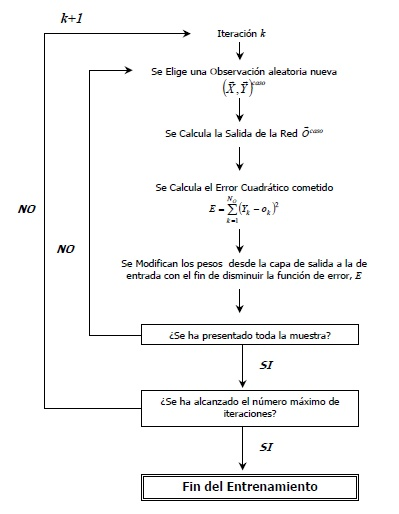
\includegraphics[scale=1.1]{Pic/diagramaentren}
	\caption{Esquema de propagación hacia atrás.\cite{Int10}}
	\label{09}
	\hrule
\end{figure}
%%%%%%%%%%%%%%%%%%%%%%%%%%%%%%%%%%%%%%%%%%%%%%%%%%%%%%%%%%%%
%%%%%%%%%%%%%%%%%%%%%%%%%%%%%%%%%%%%%%%%%%%%%%%%%%%%%%%%%%%%
\clearpage
\section{Base de datos del problema de clasificación}
Información del conjunto de datos:\\

Este archivo se refiere a las solicitudes de tarjetas de crédito. Todos los nombres y valores de los atributos se han cambiado a símbolos sin sentido para proteger la confidencialidad de los datos.\\
Este conjunto de datos es interesante porque hay una buena combinación de atributos: continuo, nominal con un pequeño número de valores y nominal con un mayor número de valores. También hay algunos valores faltantes.\\

\begin{figure}[h]
	\centering
	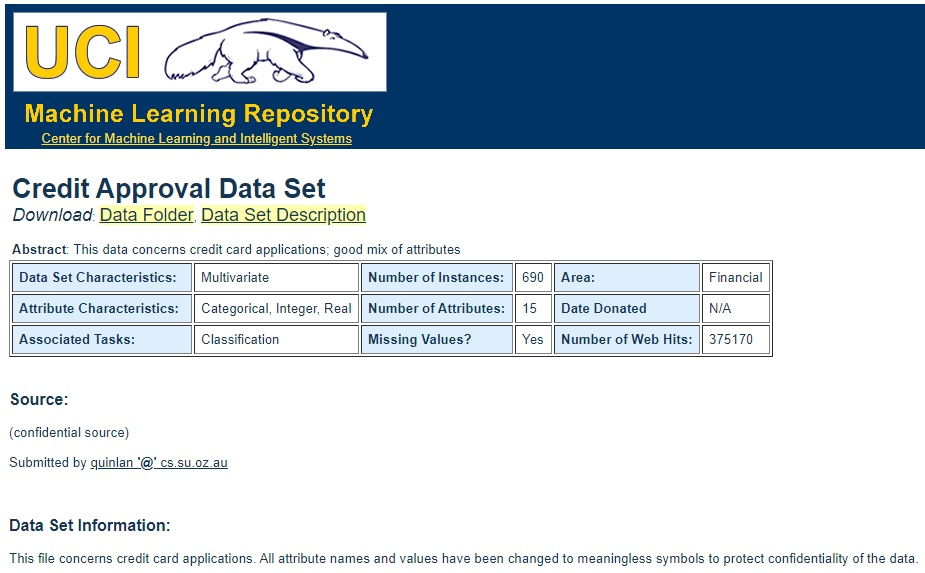
\includegraphics[scale=0.6]{Pic/Web_DB}
	\caption{Base de datos UC Irvine Machine Learning Repository \ref{07}}
	\hrule
\end{figure}

% ********************************************
% **********************************

\newpage
\thispagestyle{empty}
\vspace*{8cm}
\textbf{Euclides:\\}
\begin{center}
\textit{Las leyes de la naturaleza no son más que los pensamientos matemáticos de Dios.}
\end{center}


% ********************************************
% **********************************
\end{document}
